\graphicspath{{./chapters/operationalizing-forecasts/}}
\chapter{Operationalizing evolutionary forecasts: \evofr\ and \forecastsNcov}

In this chapter, we develop and discuss two software tools \evofr\ and \forecastsNcov\ which simplify the development, application, and communication of variant fitness dynamics and evolutionary forecasts.

\section{Introduction}

The dissertation emphasizes integrating theoretical and practical approaches, blending mechanistic insights with statistical models.
While earlier chapters focused on developing, evaluating, and applying specific models, these methods used in specific analyses motivated by existing scientific problems.
However, there is a common structure in the methods described that enables us to simplify the workflow of using these kinds of models.
In this way, we move from scientific analyses to reproducible, scalable, and applied analyses that can tackle broad questions in evolutionary forecasting. % TODO: Addressing real-time analysis
Having infrastructure for building, applying, and interpreting models allows us to iterate on our analyses, speeding up our responses and addressing real-world challenges.

% TODO: We should talk about the interest in understanding global trends for vaccine strain selection, for variant classification, and monitoring

%TODO: Expand on what it means to operationalize

\evofr\ consolidates and expands on the methods developed in this dissertation, enabling reproducible data analysis within a modular structure that allows rapid testing and comparison between models. %TODO: Reframe.
This package serves as the computational backbone for the analyses presented in this dissertation, integrating models from statistical tracking to mechanistic forecasting and is the bridge between the theoretical insights developed in this dissertation and their practical utility as an open-source tool. 

\forecastsNcov\ incorporates \evofr\ into an automated workflow and public-facing platform, translating research and applied forecasts into actionable insights for public consumption.
It continually retrieves publicly available sequence data to generate and visualize forecasts of SARS-CoV-2 variant frequencies for public consumption, providing forward-looking approach to the evolution of SARS-CoV-2 as a companion to Nextstrain. \cite{Hadfield2018}
In this way, \forecastsNcov\ serves as first step to operationalized evolutionary forecasting in practice and at scale.

Together, these software tools provide a basis for evolutionary forecasts as a dynamic process and concrete problem, setting the stage for continued development of this practice and scientifically-informed forecasts of pathogen evolution.

\section{\evofr: A toolkit for evolutionary forecasting}

Evolutionary forecasting plays a critical role in understanding genetic changes in populations over time, with direct applications in predicting the prevalence of infectious disease variants, guiding vaccine development, and informing public health interventions.

Existing tools for understanding evolution often operate at the level of phylogenetic tree estimation which is computationally expensive due to the large number of possible trees (which grows super-exponentially in terms of the number of samples).
Further, these methods have shown difficulty scaling to large numbers of sequences, requiring approximation-based methods at the pandemic scale. \cite{DeMaio2023}
Additionally, due to these large computational demands, it can be difficult to iterate on these methods, making model development, testing, and iteration time-consuming.
In general, these methods are typically employed for historical analyses, capturing past or currents trends in evolution without much concern for likely future population change.
That being said, there is no need to completely replace phylogenetic analysis as it still forms an important backbone for our understanding of pathogen evolution and enables us to group continuous genetic diversity in pathogen populations to variant groupings that are evolutionarily meaningful.
%TODO: What do I cite here.

This suggests a need to supplement phylogenetic analysis with fast, scalable, reproducible methods for analyzing sequence data at a coarse scale that can be employed for both historical and forward-looking analyses.
To address these gaps, we have developed \evofr.

\evofr\ is a Python package built for evolutionary forecasting of genetic variants, addressing the growing need for robust tools to analyze and predict change in genetic variation in real time.
With applications in evolutionary biology, epidemiology, and public health, \evofr\ integrates data pre-processing, modeling techniques, intuitive visualization tools, and a modular framework to empower researchers and scientists to understand and anticipate the dynamics of genetic variation.
It seeks to simplify bespoke analyses and allow easy integration in standardized workflows, enabling reproducible and scalable analyses.

The package facilitates data preprocessing, evolutionary forecasting, and result visualization, catering to complex datasets like those generated by genomic surveillance of pathogens (e.g., SARS-CoV-2 and influenza). 
By leveraging modularity, \evofr\ ensures scalability and extensibility, enabling users to adapt the tool for varied biological and computational challenges. 
The key contributions of this package include:
\begin{itemize}
	\item \textbf{Forecasting dynamics of genetic variants}: \evofr\ allows users to estimate the relative fitness and future prevalence of genetic variants using customizable modeling approaches such multinomial logistic regression (MLR), renewal-equation based models, Gaussian processes, and latent factor models among others.
	% \item \textbf{Bridging Data and Decision-making}:
	% 	\evofr provides researchers and decision-makers with clear, actionable visualizations of evolutionary dynamics to inform policy and intervention strategies.
	\item \textbf{Extensibility and Accessibility:} \evofr\ provides a user-friendly, open-source framework that integrates seamlessly with Python’s ecosystem, encouraging contributions and customization.
	\item \textbf{Modularity and Reproducibility} \evofr\ promotes reproducible science by offering a modular architecture that supports continued methods development, rapid iteration, model comparison, and simple integration into forecasting workflows.
\end{itemize}

\subsection{Design and implementation}

The design and implementation of \evofr\ reflect its dual purpose as a research product and public health tool.
This section will describe the software's architecture and key features, highlighting its modular design, integration of diverse modeling approaches, interchangable inference methods.

\paragraph{Modularity}

\evofr\ is divided into distinct modules for data preprocessing (\texttt{evofr.data}), modeling (\texttt{evofr.models}), inference (\texttt{evofr.infer}), and visualization (\texttt{evofr.plotting}).
Each module performs specific tasks and is designed to be interoperable.
As an example, this enables easily swapping between different models such as standard MLR, a Gaussian process-based model on the same pre-processed data.
These models can then be fit with any of the inference methods in \texttt{evofr.infer} such as Markov Chain Monte Carlo (MCMC), Stochastic Variational Inference (SVI), and maximum a posteriori (MAP) estimation.
The results of these models are stored in a standardized \texttt{evofr.posterior} object which is compatible with the various plotting methods stored in \texttt{evofr.plotting}.

\paragraph{Reproducibility}

%TODO: Deterministic workflows, documentation, standardized outputs
Fundamentally, \evofr\ seeks to make the kind of bespoke analyses that are common in papers about SARS-CoV-2 and pathogen evolution reproducible.
It contains well-documented reproductions of several methods employed in research papers, to improve the reach of these methods and enable easy replication of analyses with these papers.

While inference for these models typically involve stochastic processes, \evofr includes mechanisms to fix random seeds, ensuring that results are deterministic and consistent across runs.

Additionally, all intermediates and outputs including preprocessed data, model configurations and posterior samples can be stored in standardized formats like JSON and CSV.
This ensures that results can be reliably reproduced and shared.

\paragraph{Extensibility}

Users can extend \evofr\ by adding new models, likelihoods, or priors to the models module by developing a class that inherits from \texttt{evofr.ModelSpec}.
The package’s backend-agnostic design ensures compatibility with diverse computational frameworks (e.g., JAX, PyMC, NumPyro) since users can simply provide a log-posterior probability function for their model to enable samplng or optimization via \evofr's inference methods. \cite{jax2018github, AbrilPla2023, phan2019composable}

The plotting module (\texttt{evofr.plotting}) is built on top of matplotlib, but can be customized or replaced to accommodate specific visualization needs, such as alternative plot styles or integration with external tools. \cite{Hunter2007}

Generally, the open-source nature of \evofr\ encourages contributions, enabling the tool to evolve with user-driven innovations.

\paragraph{Scalability}

Due to most models working at the level of variant frequency, \evofr\ is designed to process genomic datasets containing thousands of sequences, with methods typically scaling with the number of variants and time-horizon for analysis.
Efficient use of computational resources and data reduction strategies ensures that analyses remain feasible as data volumes grow.
Further, integration with JAX enables just-in-time compilation and GPU/TPU acceleration for computationally intensive tasks.

\subsection{Discussion}

% State of evofr
\evofr\ is a Python-based toolkit designed to address challenges in evolutionary forecasting.
Its modular structure and emphasis on flexible workflows enable researchers to analyze and predict genetic variant dynamics.
\evofr\ is well-suited for genomic datasets generated by real-time surveillance efforts, where understanding variant dynamics is essential for public health decision-making and evolutionary monitoring.

Through its modular design, \evofr\ supports rapid iteration on models and analyses, offering tools for data preprocessing, modeling, inference, and visualization. 
By enabling reproducible workflows and fostering extensibility, \evofr\ has the potential to serve a broad range of applications, from fundamental research to forecasting in practice.

% What does evofr do
The core contributions of \evofr\ include the wide range models implemented within the package, which provide a robust foundation for exploring genetic variant dynamics under both statistical and semi-mechanistic frameworks.
By supporting customizable likelihoods and priors, \evofr\ also allows users to tailor models to specific research questions or datasets.

The package is designed to handle large genomic datasets efficiently, ensuring that \evofr\ can be applied to datasets with hundreds of thousands of sequences and extended time horizons at the national and global scale, making it ideal for real-time evolutionary forecasting.

Additionally, \evofr\ enables reproducible workflows with logging model configurations, and storing results in common formats.
These features ensure that analyses can be reliably reproduced, shared, and extended.

% Limitations 
While \evofr\ provides many significant advantages, there are some points of limitation as is.
Bayesian inference methods such as MCMC can demand significant computational resources, especially when dealing with large data sets and complex models.
  Though there are alternative, faster but approximate methods for inference such as stochastic variational inference and maximum a posteriori estimation available within the package, this still remains an issue since all inference methods may not be computational feasible for a given data set or model.

In general, the accuracy of these methods depends heavily on the quality and completeness of the data set of interest.
This means that unforeseen biases or gaps in the data can affect the reliability of these models and their predictions.
However, \evofr's extensibility will allow motivated researchers to iterate on these models to improve their ability to address such data issues.

This level of extensibility presents a potentially steep learning curve. 
Users with limited experience in probabilistic modeling may face challenges using and extended this package as is, but the documentation should provide a helpful guide for contributions looking to dive deeper.

% Future directions
In the future, we hope to expand the capabilities of \evofr\ and address the aforementioned limitations.
Further development should continue to design and implement hybrid models which combine mechanistic insight and statistical flexibility, expanding the range of questions and forms of data that \evofr\ can address and handle.
This includes additional likelihood functions and priors for extending existing models as well.

There is also a great need to eager and support contributions to \evofr\ from the open-source community.
This includes adding more thorough documentation of the package as well as the development of extended guide for contributors that is accessible to users.
Going forward, the goal should be expanding the package to meet the needs of the communities who would most benefit from it: researchers and scientists in epidemiology, evolutionary biology, and public health.

% Broader impacts
\evofr\ democratizes evolutionary forecasting by turning statistical methods developed for research to a practical, scalable, and accessible tools for analysis.
This positions \evofr\ as a useful for real-time applications in public, such as monitoring emerging variants or informing vaccine development.

Beyond its immediate applications, \evofr\ serves as a model for the development of modular, extensible tools in computational biology.
Its design and implementation demonstrate the utility of combining reproducibility, scalability, and user-centered design to address complex challenges in research. 
By bridging the gap between theoretical models and practical applications, \evofr\ sets the stage for continued advancements in evolutionary forecasting and beyond.

\subsection*{Code availability}

\evofr\ is an open source project.
Its source code can be found at \href{https://github.com/blab/evofr}{https://github.com/blab/evofr}.
Its documentation can be found at \href{https://blab.github.io/evofr}{https://blab.github.io/evofr}.

\section{\forecastsNcov: Automated and public-facing forecasts for SARS-CoV-2}


\forecastsNcov\ is an automated platform designed to provide real-time forecasts of SARS-CoV-2 variant frequencies.
As part of the broader Nextstrain project, it extends Nextstrain’s genomic surveillance capabilities by offering a forward-looking perspective. \cite{Hadfield2018}
While Nextstrain’s phylogenetic inference provides detailed reconstructions of evolutionary histories, \forecastsNcov\ complements this by projecting future variant trajectories.
This dual approach ensures a comprehensive understanding of variant dynamics, bridging retrospective insights with predictive capabilities.

This tool operationalizes evolutionary forecasting, translating genomic data into actionable insights for public health.
Its automated workflows, robust modeling framework, and accessible visualization tools make it an essential resource for addressing rapidly evolving public health challenges.
By enabling real-time forecasting, \forecastsNcov\ can support early detection of emerging threats, timely policy decisions, and informed vaccine updates.

% \forecastsNcov\ is an automated workflow that processes SARS-CoV-2 sequence data, processes these into a sharable format, applies \evofr’s forecasting models, and visualizes their results in a web interface, providing real-time insights into SARS-CoV-2 variant dynamics.
% \forecastsNcov\ uses publicly submitted genomic data, to produce variant frequency forecasts and variant-specific growth advantages to monitor and nowcast SARS-CoV-2 variant dynamics, directly complementing Nextstrain’s phylogenetic analyses by adding predictive, forward-looking insights.
% \forecastsNcov\ forecasts variant trajectories (e.g., growth advantage, frequency) alongside phylogenetic data from Nextstrain to provide a comprehensive view of virus evolution. This strengthens Nextstrain’s ability to not only visualize past evolutionary relationships but also predict future trends in variant dynamics. %TODO: Correct this heavily. We want to describe this as a frequency-based complement to 

% \forecastsNcov enhances this by predicting the future dynamics of viral variants based on their evolutionary and fitness characteristics.
% While Nextstrain focuses on tracking past evolutionary trends, \forecastsNcov\ looks forward, using statistical and mechanistic models to forecast how variants will evolve over time.

%TODO: Add Figures: Clade level frequencies and growth advantages, lineage growth advantages
% Be sure to caption data last updated

% TODO: Why it's useful for these things to be integrated 
\subsection{Design and workflow}

The \forecastsNcov\ pipeline integrates data ingestion, predictive modeling, and visualization into a seamless, automated workflow.
It is designed to operate at scale, updating forecasts daily to provide consistent and timely insights.

% This is where we discuss automated sequence count generation, the workflow for country-level fitness at multiple levels of genetic variation.
Data ingestion is handled by workflows that retrieve and preprocess genomic data from public repositories, such as GISAID and GenBank, using the Nextstrain \texttt{ncov-ingest} pipeline.
These workflows ensure high-quality, curated inputs by harmonizing metadata and sequence information across multiple sources.
This generates sequence count files at various levels of genetic granularity (Nextstrain clade and Pango lineage), geographic resolution (Global and the United States) from data.

Forecasting is performed using predictive models implemented in \evofr\.
These models estimate key parameters such as variant frequencies, growth rates, and fitness advantages, generating forward-looking insights that complement traditional phylogenetic analyses.
By focusing on coarse-scale trends, the platform prioritizes actionable predictions over detailed evolutionary reconstructions.
Though compatible with any model from \evofr\, live forecasts rely on an in-house hierarchical multinomial logistic regression model.

% We can also talk about the web-app for simplified visualization.
The visualization component transforms model outputs into interactive, web-based visualizations that present variant trajectories in accessible formats.
%TODO: Change to say that it enables easy visualization of \evofr's outputs for web applications.
%TODO: Mention that we host a website and provide the link
This web application allows users to explore the latest forecasts or upload local data for analysis.
These visualizations provide intuitive representations of complex genomic data, making \forecastsNcov a valuable resource for technical and non-technical audiences alike.

\subsection{Contributions}

As a component of Nextstrain, \forecastsNcov fills a critical gap by adding predictive capabilities to the platform’s established phylogenetic tools.
It provides continuously updated forecasts that enable users to anticipate the trajectories of SARS-CoV-2 variants (Figs \ref{fig:fn_clade_frequencies} and \ref{fig:fn_lineage_frequencies})  as well as visualize the current growth advantages of variants at the level of Nextstrain clade and Pango lineage (Figs \ref{fig:fn_clade_growth_advantages} and Figs \ref{fig:fn_lineage_growth_advantages}).

This forward-looking approach complements the retrospective focus of phylogenetic inference, creating a comprehensive framework for understanding both past and future variant dynamics.

By automating the forecasting process, \forecastsNcov ensures the timely availability of results, which are stored publicly as JSON files on AWS S3.
These outputs are stratified by data provenance (e.g., GISAID, GenBank), variant classification (e.g., Nextstrain clades, Pango lineages), and geographic resolution (e.g., global, USA).
The integration of these outputs with an interactive web application further enhances their accessibility, enabling users to visualize variant trends dynamically.
This functionality supports public health efforts by providing actionable insights that inform decision-making at local, national, and global levels.

\subsection{Discussion}

\forecastsNcov\ represents a significant advancement in operationalizing evolutionary forecasting, combining the predictive modeling framework of \evofr with Nextstrain’s robust infrastructure for genomic surveillance.
By automating the end-to-end process—from data ingestion to real-time forecast visualization—the platform offers a forward-looking complement to the phylogenetic analyses that form the foundation of Nextstrain.
This dual approach provides a more comprehensive understanding of variant dynamics, addressing both retrospective and prospective dimensions of pathogen evolution.

The platform’s success lies in its ability to integrate predictive models seamlessly into a scalable pipeline that produces actionable outputs.
These forecasts have proven particularly valuable for tracking SARS-CoV-2 variants, enabling public health agencies to anticipate potential surges and prioritize interventions.
By presenting outputs through intuitive visualizations and accessible data formats, \forecastsNcov\ democratizes access to evolutionary insights, fostering collaboration among researchers, public health professionals, and policymakers.

However, real-time forecasting brings unique challenges that merit consideration.
The reliance on external data sources, such as GISAID and GenBank, introduces dependencies that can affect the timeliness and consistency of updates.
Additionally, the variability in global sequencing efforts can create gaps or biases in the underlying data, which in turn may influence forecast accuracy.
While the platform’s modular design supports customization and iteration to address such issues, these constraints highlight the ongoing need for robust data-sharing practices and equitable genomic surveillance.

Another area of consideration is the interpretability of forecasts.
While visualizations simplify complex data, conveying the uncertainties inherent in predictive models remains challenging, particularly for non-technical audiences.
Enhancing these aspects would strengthen \forecastsNcov\ as a tool for decision-making, ensuring that forecasts are not only accessible but also actionable.

Looking ahead, the scalability and extensibility of \forecastsNcov\ provide a strong foundation for future growth.
The platform is well-positioned to expand its scope to other pathogens, offering similar predictive capabilities for influenza, RSV, and other emerging threats.
Further development of its visualization tools could enable deeper engagement with forecast data, while continued integration with Nextstrain’s ecosystem would create an increasingly unified platform for genomic epidemiology.

Ultimately, \forecastsNcov\ exemplifies the potential of evolutionary forecasting to move beyond research applications and into the realm of real-world impact.
By providing timely and actionable insights, the platform underscores the value of combining computational innovation with public health priorities, setting the stage for further advancements in genomic surveillance and predictive modeling.

\subsection*{Code availability}

\forecastsNcov\ is an open source project.
Its source code can be found at \href{https://github.com/nextstrain/forecasts-ncov}{https://github.com/nextstrain/forecasts-ncov}.
The live SARS-CoV-2 forecasts can be found at \href{https://nextstrain.org/sars-cov-2/forecasts}{https://nextstrain.org/sars-cov-2/forecasts}.

\begin{figure}[h]
    \centering
    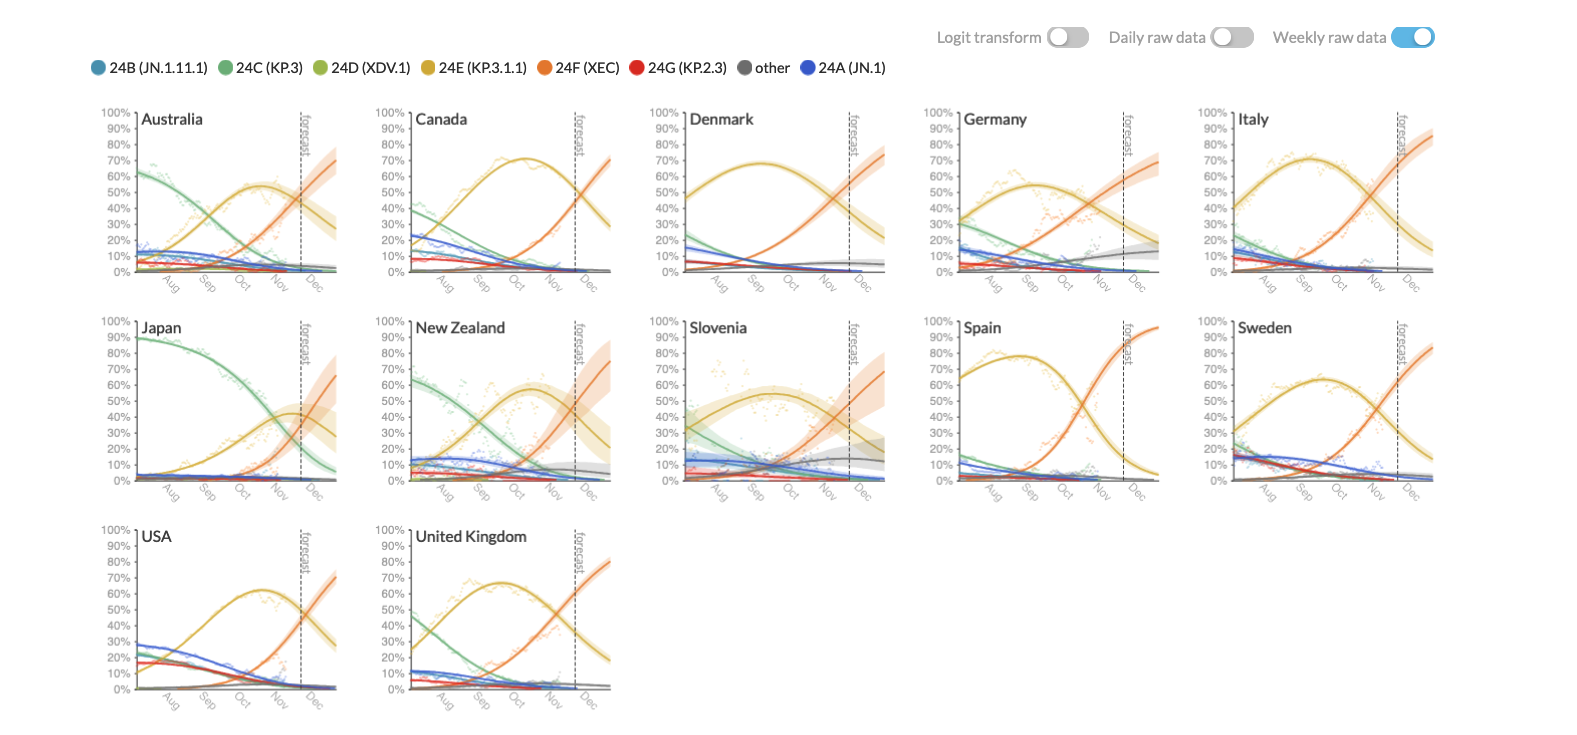
\includegraphics[width=1.0\linewidth]{./figures/clade_frequencies.png}
    \caption{
      \textbf{Live global SARS-CoV-2 frequency forecasts for Nextstrain clades.}
    }
    \label{fig:fn_clade_frequencies}
\end{figure}


\begin{figure}[h]
    \centering
    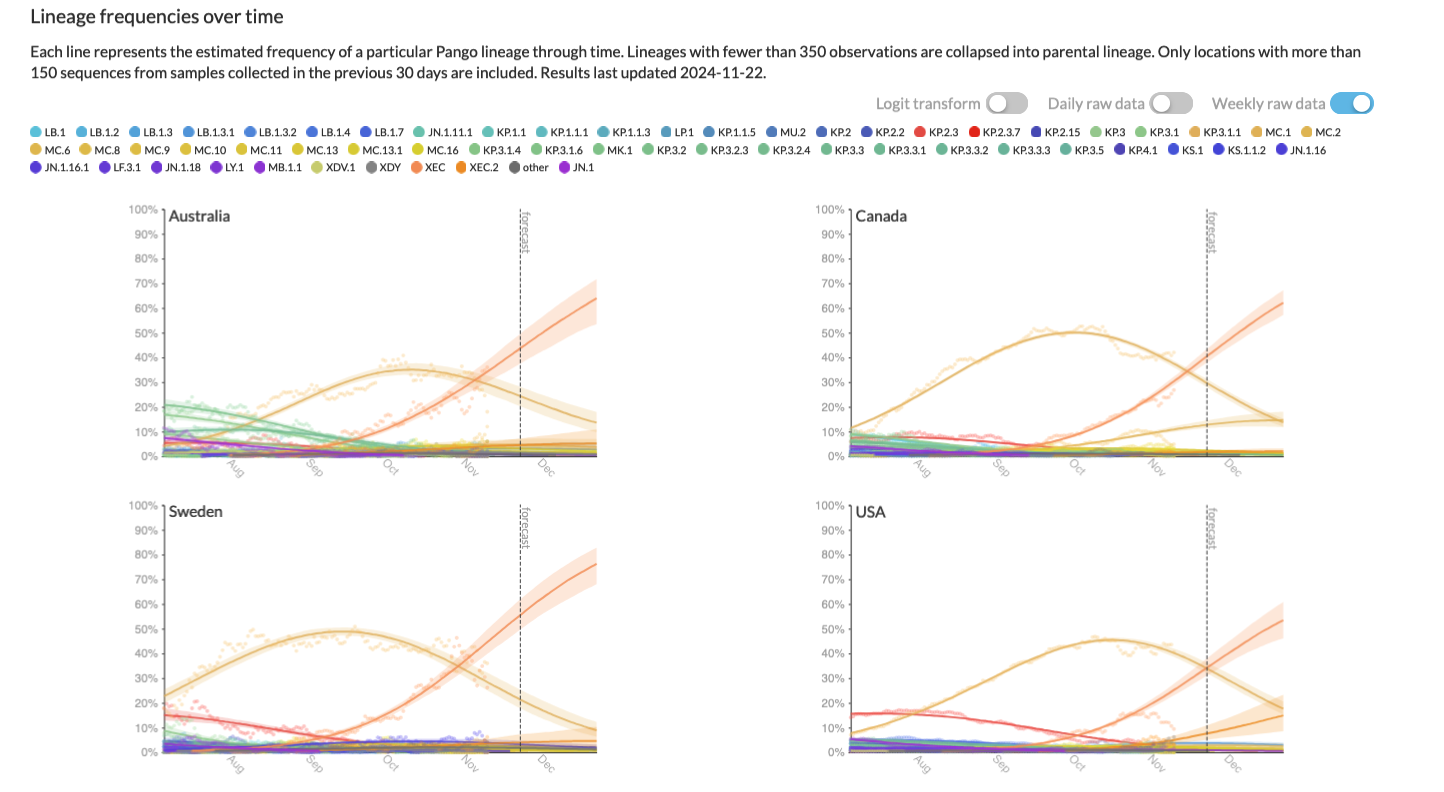
\includegraphics[width=1.0\linewidth]{./figures/lineage_frequencies.png}
    \caption{
      \textbf{Live global SARS-CoV-2 frequency forecasts for Pango lineages.}
    }
    \label{fig:fn_lineage_frequencies}
\end{figure}


\begin{figure}[h]
    \centering
    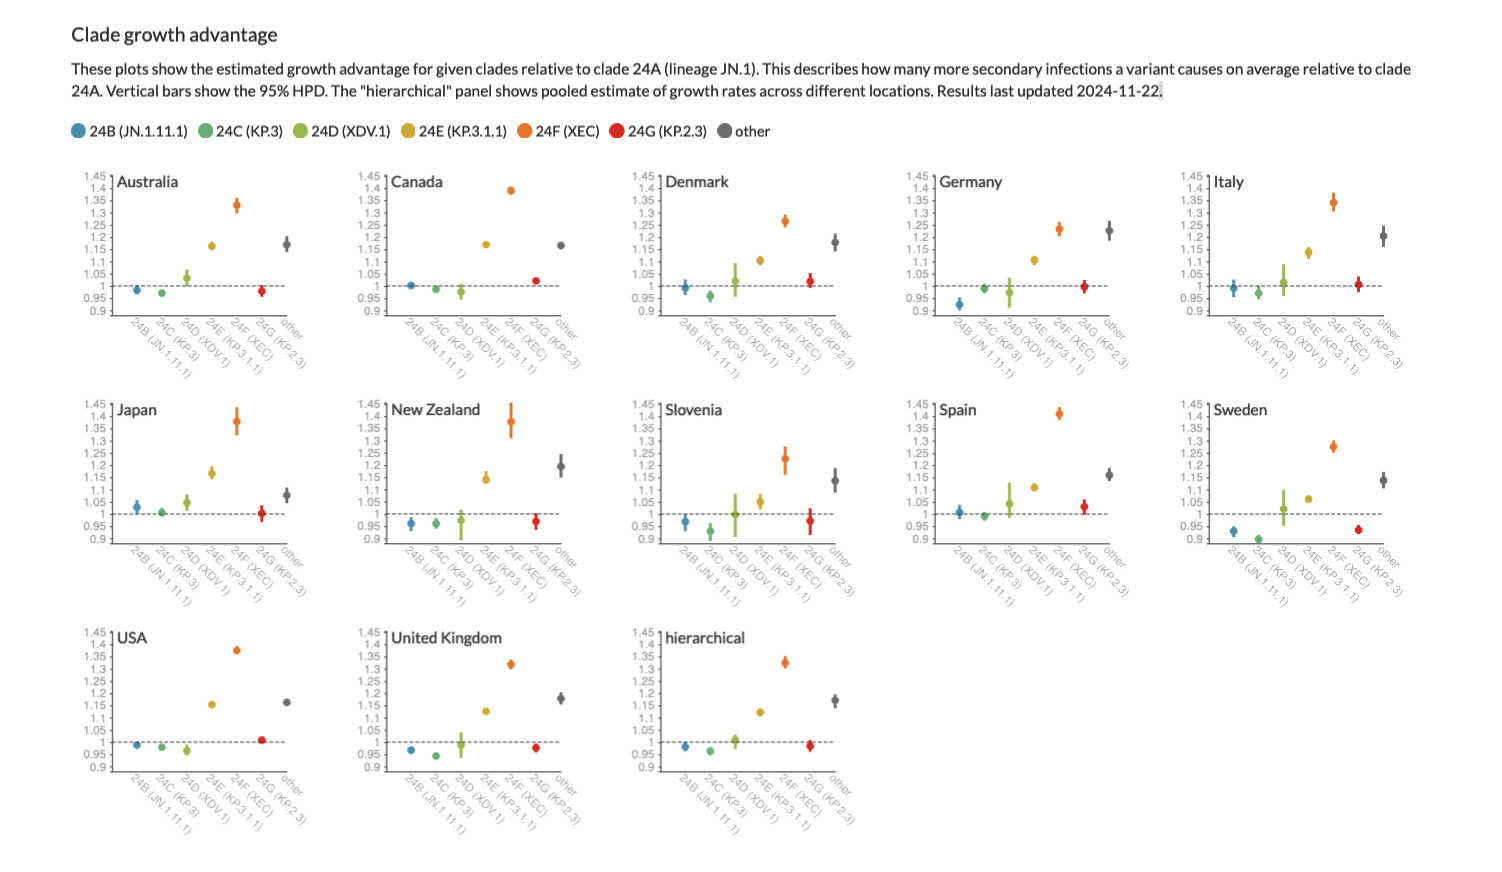
\includegraphics[width=1.0\linewidth]{./figures/clade_growth_advantages.png}
    \caption{
      \textbf{Live global SARS-CoV-2 growth advantage estimates for Nextstrain clades.}
    }
    \label{fig:fn_clade_growth_advantages}
\end{figure}


\begin{figure}[h]
    \centering
    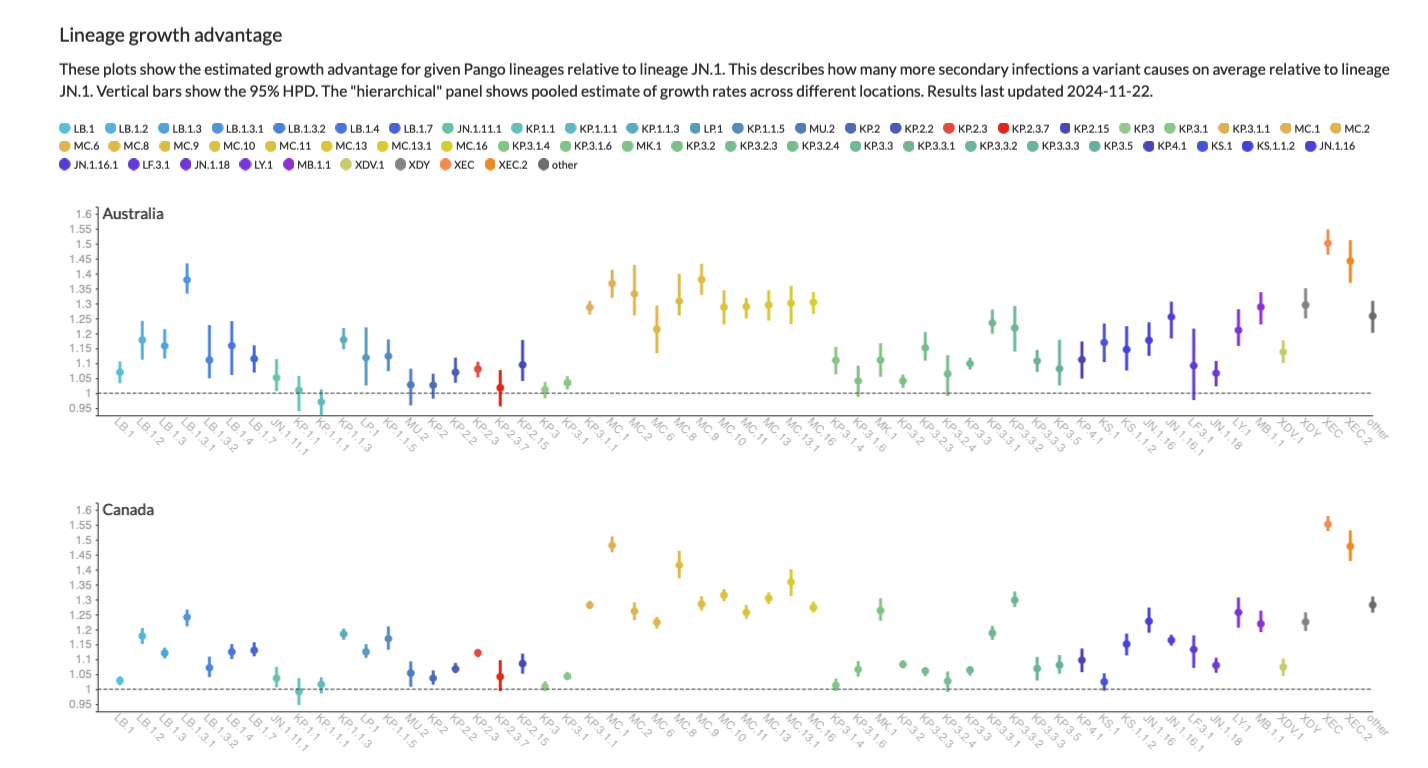
\includegraphics[width=1.0\linewidth]{./figures/lineage_growth_advantages.png}
    \caption{
      \textbf{Live global SARS-CoV-2 growth advantage estimates for Pango lineages.}
    }
    \label{fig:fn_lineage_growth_advantages}
\end{figure}
